\section{Grappa} \label{sec:grappa}

\begin{figure}[t]
\begin{center}
  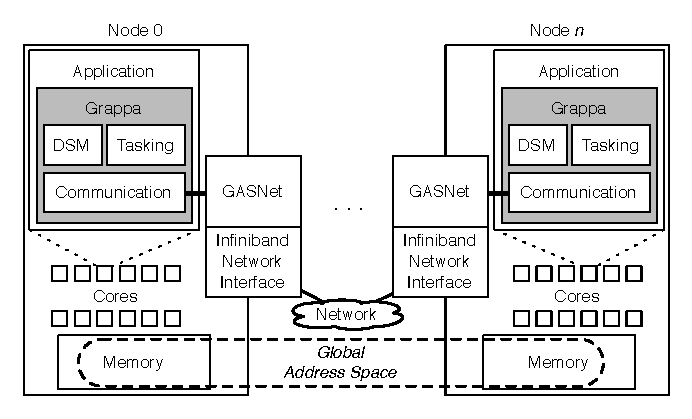
\includegraphics[width=0.95\columnwidth]{figs/system-overview}
\begin{minipage}{0.95\columnwidth}
  \caption{\label{fig:grappa} Grappa system overview}
\end{minipage}
\vspace{-3ex}
\end{center}
\end{figure}

The Grappa runtime system (Figure~\ref{fig:grappa}) supports scaling of irregular applications via three key components:
a \textbf{distributed shared global memory} providing high aggregate random access bandwidth for both normal and synchronized operations;  
a \textbf{tasking system} with lightweight multithreading to tolerate latency and workstealing to automate load balance;
and a \textbf{communication layer} using network packet scheduling and aggregation to achieve high performance while remaining largely invisible to applications.
Unlike many runtime systems where the task scheduler, memory access manager, and the communication  are separable subsystems, in Grappa these three components are tightly integrated and the performance of each depends heavily on that of the other two.  For example, eficiency of the communication layer requires that the tasking system multiplex tasks -- and the memory manager fetch data -- sufficiently rapidly to aggregate hundreds of individual requests into each packet; otherwise, the network will be poorly utilized.  Nonetheless, for simplicity of exposition, we describe each component in turn.

We now discuss the
programmer's view of Grappa's main capabilities, including a subset of
the Grappa API. In Section~\ref{implementation}, we discuss the details
of their implementation.

\TODO{Should we have a code example here, and walk thru it as we explain the
components and parts of the API?}

\subsection{Tasks}

%The basic unit of locality in Grappa is the {\em core}. Each core is
%responsible for a section of the global memory

The basic unit of execution in Grappa is a {\em task}. Tasks are
small; just a function pointer and arguments. Tasks are only
queued when they are spawned; later, when resources are free, they are
allocated a stack, bound to a core, and executed.

Grappa's tasks give up control of their core when when they perform
long-latency operations, allowing the processor to remain busy while
waiting for the operation to complete. This is most often done
implicitly inside a call into Grappa's API, but it can also be done
explicitly by the programmer using the calls shown in
Figure~\ref{fig:scheduling}. \TODO{cite UPC split phase reads and
writes, but include that we provide a way to overlap computation}

All Grappa scheduling is done in userspace, and minimal state is saved,
in order to minimize the context switch time. In our experiments, we saw
context switch times as low as \checkme{40ns}. This lightweight context
switching is Grappa's key enabling feature. It gives us the ability to
tolerate latency. Given that ability, we are able to \textbf{trade
latency for throughput}: by {\em increasing} latency in key components
in the system we are able to increase our aggregate random access
bandwidth, our synchronization bandwidth, and our ability to tolerate
load.

\begin{figure}[htbp]
  \begin{center}
    \begin{description}\small
    \item[ \texttt{ yield() } ] \hfill \\
      Gives up control of core to scheduler, queuing task to be scheduled again soon
    \item[ \texttt{ suspend() } ] \hfill \\
      Gives up control of core to scheduler
    \item[ \texttt{ wake( task * $t$ ) } ] \hfill \\
      Enqueues $t$ to be scheduled again soon
    \end{description}
    \begin{minipage}{0.95\columnwidth}
      \caption{\label{fig:scheduling} Grappa API: scheduling} %{-4ex}}
    \end{minipage}
    %\vspace{-3ex}
  \end{center}
\end{figure}


\subsection{Expressing parallelism}

A programmer's goal in coding with Grappa should be to express as much
parallelism as possible without worrying about where it will execute.
Grappa then chooses where and when to exploit this parallelism,
scheduling as much work as necessary to tolerate network latencies and
keep cores busy. 

Grappa provides four methods for expressing parallelism, shown in
Figure~\ref{fig:expressing-parallelism}. The first is explicit task
spawns. When the programmer identifies work that can be done in
parallel, the work may be wrapped up in a function and queued with its
arguments for later execution using a \texttt{spawn}. If the
programmer wishes to spawn a task on a specific core in the system,
or at the home core of a particular memory location, Grappa provides a
\texttt{spawn\_on} call for this purpose.

The next method for expressing parallelism is a parallel for loop, where
the number of iterations must be known at loop entry. The programmer
specifies a function pointer along with start and end indices and an
optional threshold to control parallel overhead. Grappa does {\em
recursive decomposition} of iterations, similar to Cilk's cilk\_for
construct~\cite {cilkforimplementation} \comment{could only find slides
page6 of
http://www.clear.rice.edu/comp422/lecture-notes/comp422-2012-Lecture5-
Cilk++.pdf    ---- Good enough.  Cite it.  -Mark}.  It generates a
logarithmically-deep tree of tasks, stopping to execute the loop body
when the number of iterations is below the required threshold. Finally,
a programmer may want to run a small piece of code on a particular core
in the system without waiting for execution resources to be available.
Grappa provides the \texttt{call\_on} call for this purpose.

\begin{figure}[htbp]
  \begin{center}
    \begin{description}\small
    \item[ \texttt{spawn( void (*fp)(args) )} ] \hfill \\
      Creates a new stealable task
    \item[ \texttt{spawn\_on( core, (*fp)(args) )} ] \hfill \\
      Creates a new private task that will run on a specific core 
    \item[ \texttt{parallel\_for( (*fp)(args), start, end )} ] \hfill \\
      Executes iterations of a loop as stealable tasks 
    \item[ \texttt{call\_on( core, (*fp)(args) )} ] \hfill \\ 
      Runs a limited function on a specific core without consuming
      Grappa execution resources 
    \end{description}
    \begin{minipage}{0.95\columnwidth}
      \caption{\label{fig:expressing-parallelism} Grappa API: expressing parallelism} % \vspace{-4ex}}
    \end{minipage}
    %\vspace{-3ex}
  \end{center}
\end{figure}

\subsection{Memory}

Applications written for Grappa utilize two forms of memory: local and
global.

Local memory is local to a single core in the system.  Accesses occur
through conventional pointers.  The compiler emits an access and the
memory is manipulated directly.  Applications use local accesses for a
number of things in Grappa: the stack associated with a task, accesses
to localized global memory in caches (see below), and accesses to
debugging infrastructure that is local to each system node.  Local
pointers cannot access memory on other cores, and are valid only on
their home core.

Large data that is expected to be shared and accessed with low locality is
stored in Grappa's global memory. All global data must be accessed through
calls into Grappa's API, shown in Figure~\ref{fig:accessing-memory}.

\paragraph{Global memory allocation}
Grappa provides two methods for {\emph storing} data in the global memory. The
first is a distributed heap striped across all the machines in the
system. The \texttt{global\_malloc} and \texttt{global\_free} calls
are used to allocate and deallocate memory in the global heap; on
allocation, a global pointer is returned. Grappa also allows any local
data on a core's stacks or heap to be exported to the global address
space to be made accessible to other cores across the system.

\paragraph{Global memory access} There are two approaches to {\emph
accessing} global memory. When the programmer expects a computation on
shared data to have spatial locality to exploit, {\em cache} operations
may be used. When there is no locality to exploit, {\em delegate}
operations are used. Since these operations are expected to communicate
with other nodes and have high latency, cache and delegate operations
interact with the scheduler; when issuing a long-latency request, they
suspend the requesting task and allow the core to execute other work
until their response arrives.

\paragraph{Explicit caching} With Grappa's explicit caching support,
applications can instruct Grappa to fetch a global pointer of any length
and return a local pointer to a cached copy of the global memory. Under
the hood, Grappa performs the mechanics of gathering chunks of data from
multiple system nodes and presenting a conventional appearing linear
block of memory as a pointer into a cache. Grappa cache operations have
the usual read-only and read-write variants, along with a write-only
variant used to initialize data structures. Cache operations exploit
spatial locality by reducing the number of small network messages
accessing contiguous data. Languages for distributed shared memory
systems have done optimizations to achieve a similar goal. For example,
the UPC compiler coalesces struct and array accesses into remote get/put
\cite{Chen:2005}, and Fortran D compiler's message vectorization hoists
small messages out of a loop \cite{FortranD:1992}. Caching in Grappa
additionally provides a mechanism for exploiting temporal locality by
operating on the data locally. 

\paragraph{Delegate operations}
When the access pattern has low-locality, it is more efficient
to modify the data on its home core rather than bringing a copy to the
requesting core and returning it after modification. Delegate
operations provide this capability. Applications can dispatch
computation to be performed on individual machine-word sized chunks of
global memory to the memory system itself (e.g.,
\emph{fetch-and-add}). \comment{should we bring up delegation in the intro?}

Delegate operations, proposed in \cite{Nelson:hotpar11}, are also the
primary synchronization method in Grappa. Each piece of global memory is
paired with a single core in the system; all accesses to that actual
memory location are done by that core. This allows delegate operations
to be performed atomically on the core simply by making sure no other
code interleaves their operation; and, since context switches in Grappa
are cooperative, this is trivial. Thus, delegate operations are able to
provide atomic semantics to memory owned by one core without using
atomic operations. Using delegation to implement isolation for any
subset of memory has been explored in \cite{delegated:oopsla11}.

\begin{figure}[htbp]
  \begin{center}
    \begin{description}\small
      \item[ \texttt{ global\_address global\_malloc( size )} ] \hfill \\
      \item[ \texttt{ global\_free( global\_address )} ] \hfill \\
        Allocates and frees memory in the global heap
      \item[ \texttt{ delegate\_read( global\_address, local\_var )} ] 
      \item[ \texttt{ delegate\_write( global\_address, local\_var )} ] %\vspace{-2ex}
      \item[ \texttt{ delegate\_cas( global\_address, local\_var )} ] %\vspace{-2ex}
      \item[ \texttt{ delegate\_inc( global\_address, local\_var )} ] %\vspace{-2ex} 
\hfill \\
        Performs a memory operation at the home core of a global address
      \item[ \texttt{ cache\_acquire( global\_address, local\_buf, \{RO,RW,WO\})} ]
      \item[ \texttt{ cache\_release( global\_address, local\_buf )} ] %\vspace{-2ex} 
\hfill \\
        Perform cache operations \TODO{expand}
    \end{description}
    \begin{minipage}{0.95\columnwidth}
      \caption{\label{fig:accessing-memory} Grappa API: accessing memory} %{-4ex}}
    \end{minipage}
    %\vspace{-3ex}
  \end{center}
\end{figure}

